\begin{figure}[h!]
    \centering
    \caption{Geographic Spillovers of \emph{Plan Cuadrante} for Neighbors of the ENUSC Municipalities (Administrative Outcomes)}
    \label{fig:figure_46ENUSC_spillovers_admin}
    \begin{subfigure}{0.495\textwidth}
        \centering
        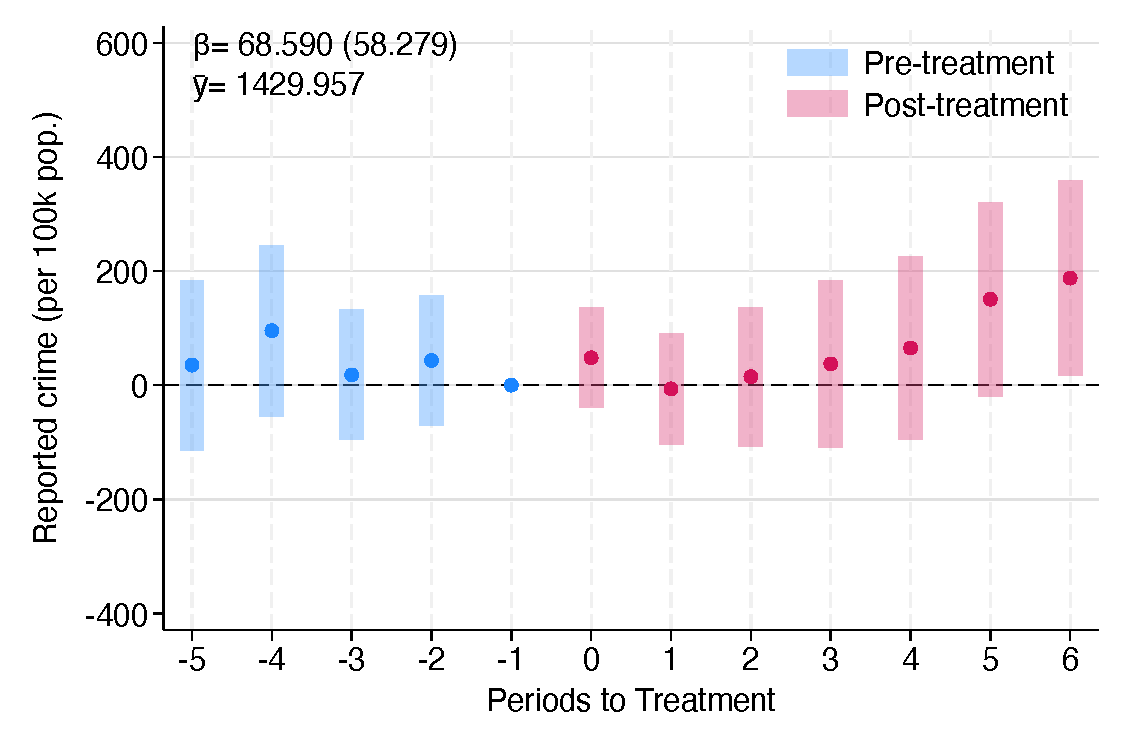
\includegraphics[width=0.98\textwidth]{../manuscript/Graphs/totalreportedcrime_enusc47_neighbors.pdf}
        \caption{Spillovers on Reported Crime}
    \end{subfigure}%
    ~
    \begin{subfigure}{0.495\textwidth}
        \centering
        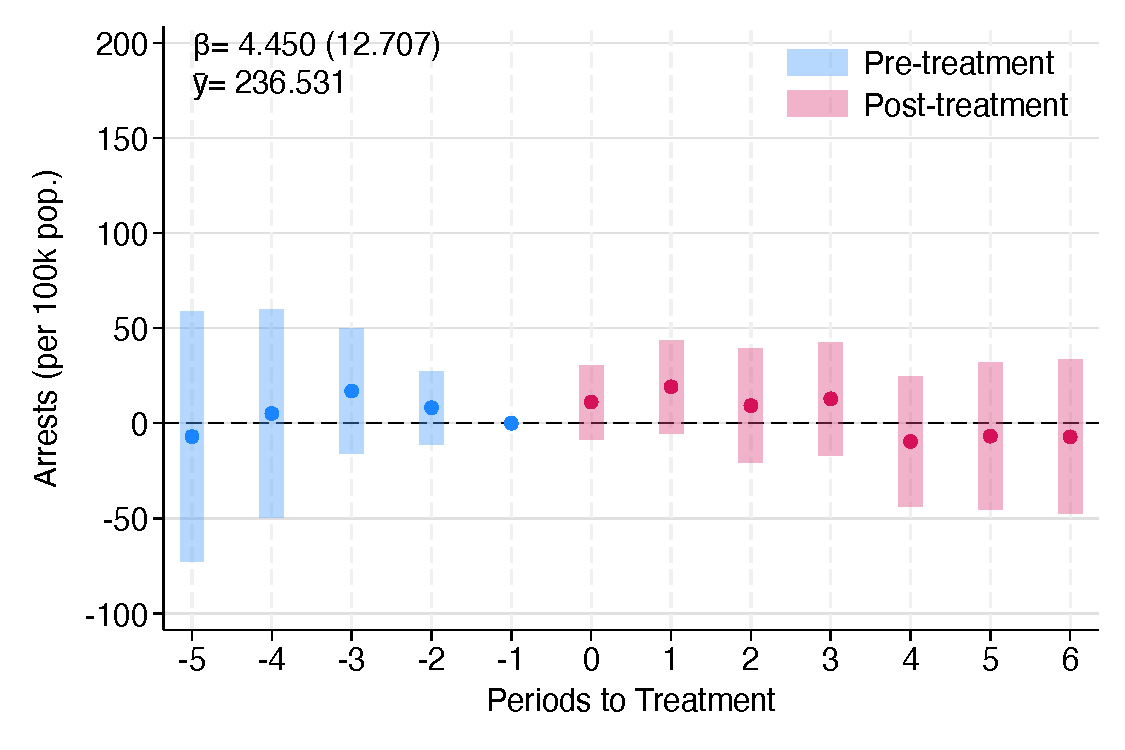
\includegraphics[width=0.98\textwidth]{../manuscript/Graphs/totalarrestscrime_enusc47_neighbors.pdf}
        \caption{Spillovers on Arrests}
    \end{subfigure}

    \vspace{0.5em}

    \begin{subfigure}{0.495\textwidth}
        \centering
        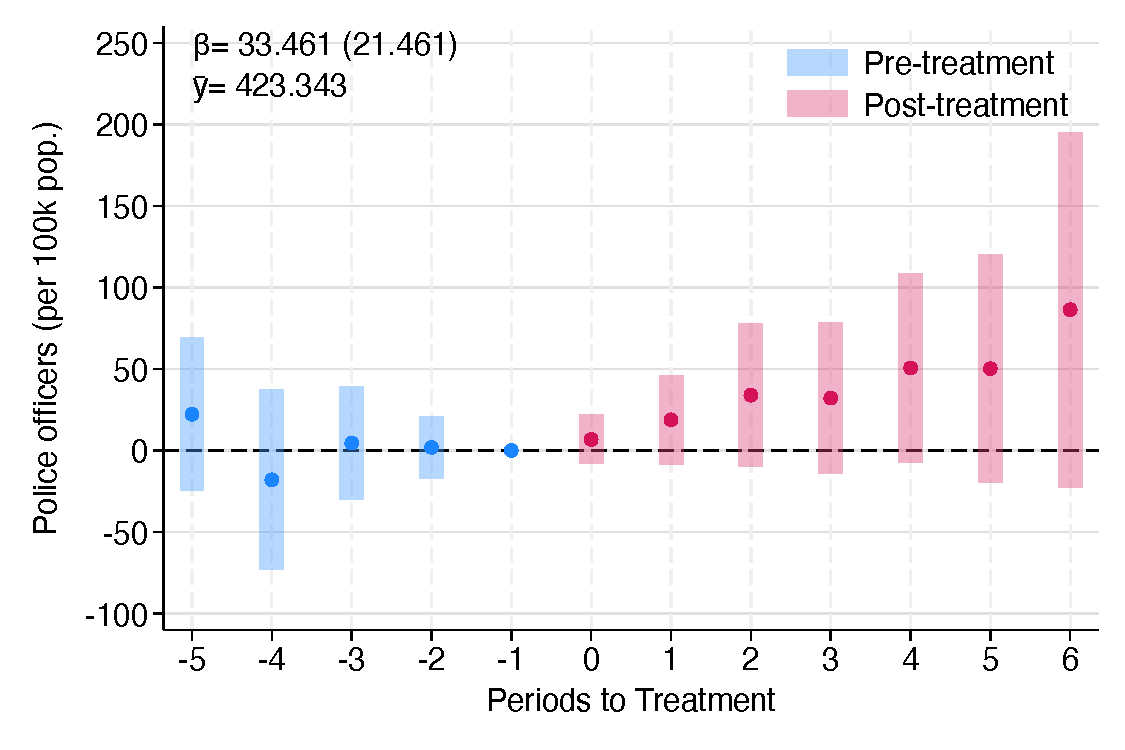
\includegraphics[width=0.98\textwidth]{../manuscript/Graphs/dotpc_enusc47_neighbors.pdf}
        \caption{Spillovers on Police Officers}
    \end{subfigure}%
    ~
    \begin{subfigure}{0.495\textwidth}
        \centering
        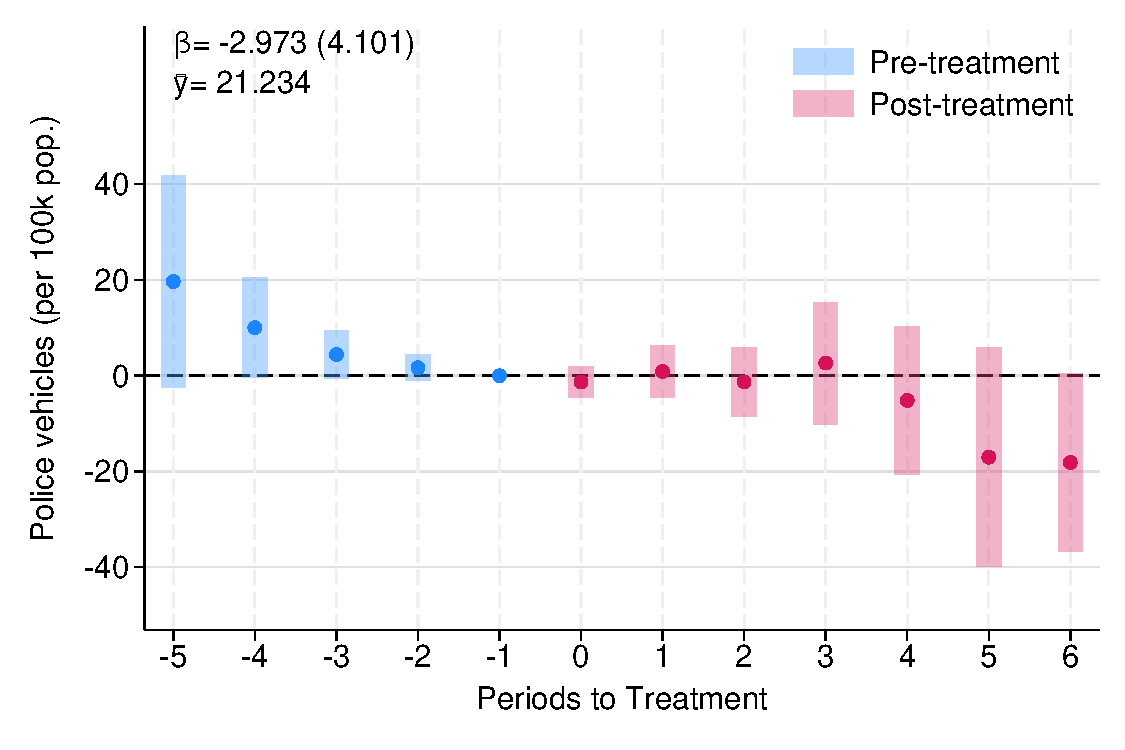
\includegraphics[width=0.98\textwidth]{../manuscript/Graphs/vehiclespc_enusc47_neighbors.pdf}
        \caption{Spillovers on Patrol Vehicles}
    \end{subfigure}

\begin{minipage}{\textwidth}
\footnotesize Notes: This figure reports the spillover effects of \emph{Plan Cuadrante} on the number of crimes reported to the police in the municipality per 100,000 inhabitants (panel a), on the number of arrests in the municipality per 100,000 inhabitants (panel b), on the number of police officers (panel c), and on the number of patrol vehicles (panel d). Specifically, the figure shows the dynamic effects of \emph{Plan Cuadrante} for neighboring never-treated municipalities to the 46 municipalities included in the ENUSC sample. The estimation is conducted using the procedure developed in \citet{Callaway} for difference-in-differences with staggered treatment adoption, using as the treatment introduction date the earliest date of a neighboring municipality. The dots in the figure represent the estimated coefficients and the bars behind them 95\% confidence intervals. Standard errors are clustered at the municipality level using the wild bootstrap procedure. The pooled effect and the mean outcome before the introduction of the treatment for each outcome are also presented in each panel.
\end{minipage}
\end{figure}


\begin{figure}[h!]
    \centering
    \caption{Geographic Spillovers of \emph{Plan Cuadrante} on ENUSC Survey Outcomes (Early- to Late-Adopting Municipalities)}
    \label{fig:figure_results_spillovers_enusc}
    \begin{subfigure}{0.495\textwidth}
        \centering
        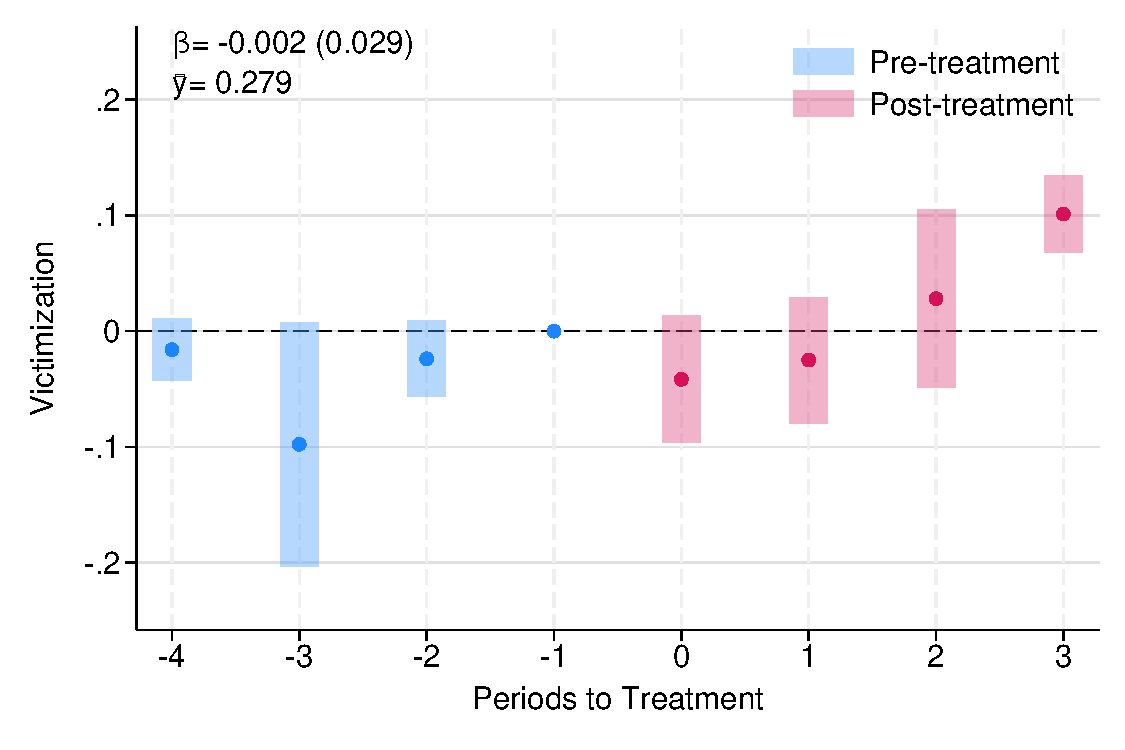
\includegraphics[width=0.98\textwidth]{../manuscript/Graphs/results_spillover_delitos.pdf}
        \caption{Spillovers on Victimization in last 12 months}
    \end{subfigure}%
    ~
    \begin{subfigure}{0.495\textwidth}
        \centering
        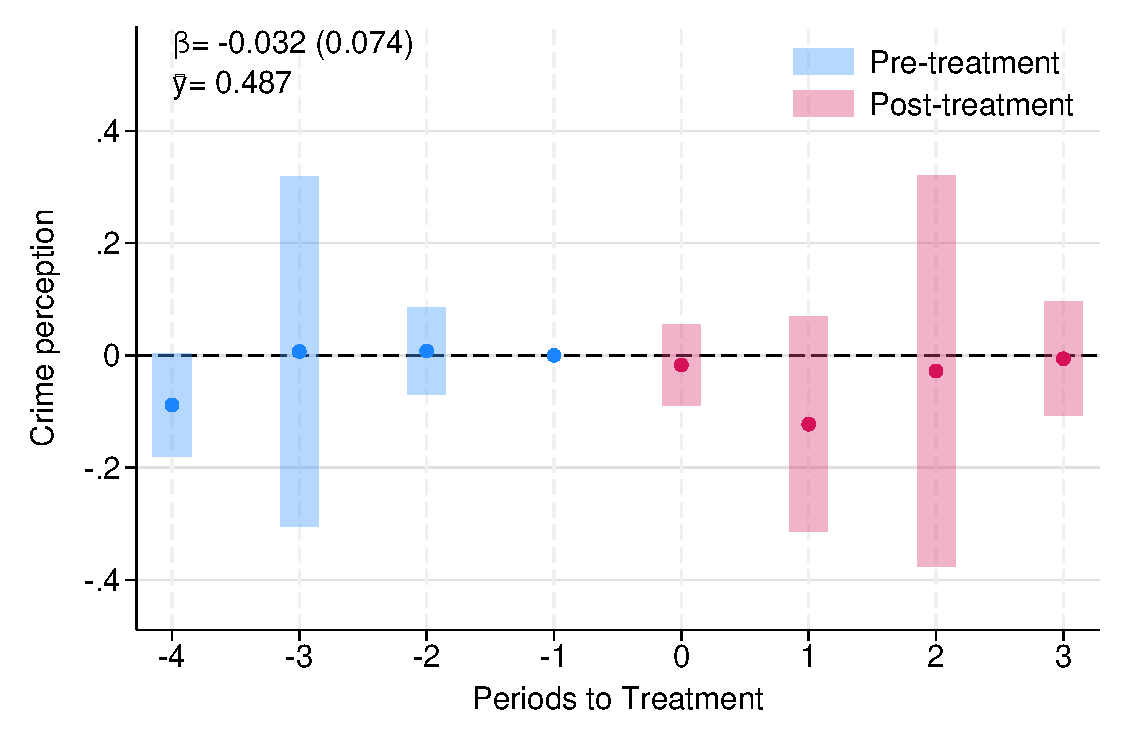
\includegraphics[width=0.98\textwidth]{../manuscript/Graphs/results_spillover_inseguridad_barrio1.pdf}
        \caption{Spillovers on Households reporting an increase in crime}
    \end{subfigure}
    \vspace{0.5em}
    \begin{subfigure}{0.495\textwidth}
        \centering
        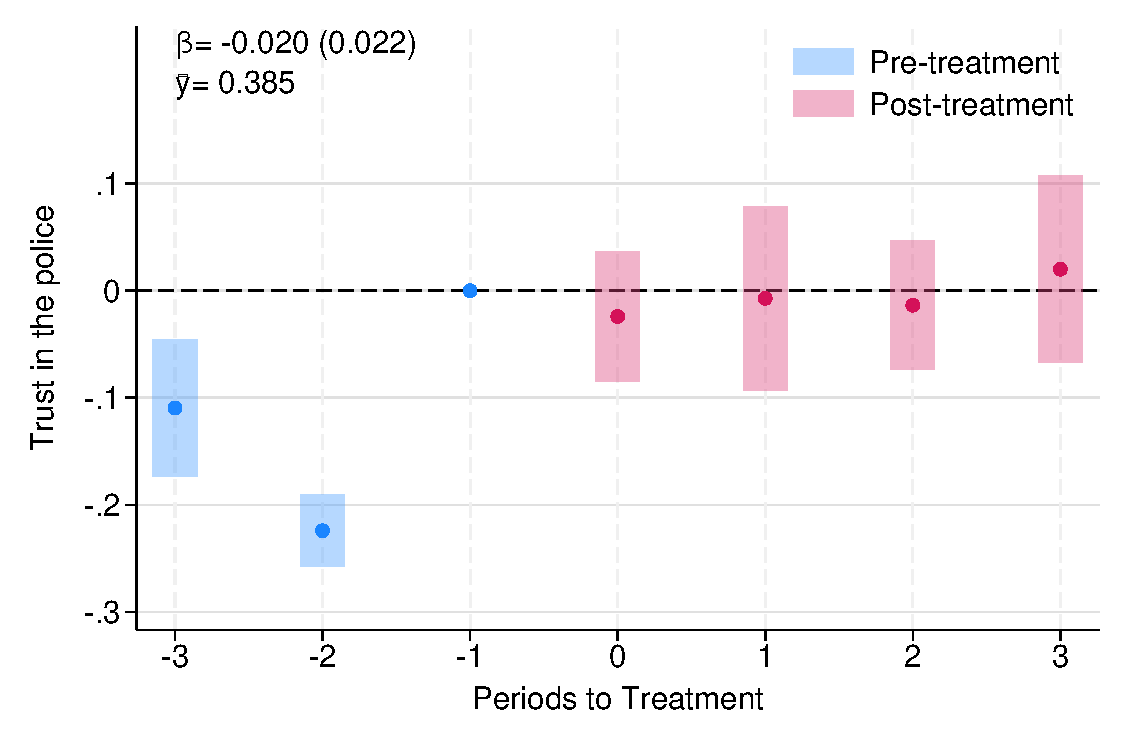
\includegraphics[width=0.98\textwidth]{../manuscript/Graphs/results_spillover_confianza_carabineros.pdf}
        \caption{Spillovers on Trust in the police}
    \end{subfigure}%
    ~
    \begin{subfigure}{0.495\textwidth}
        \centering
        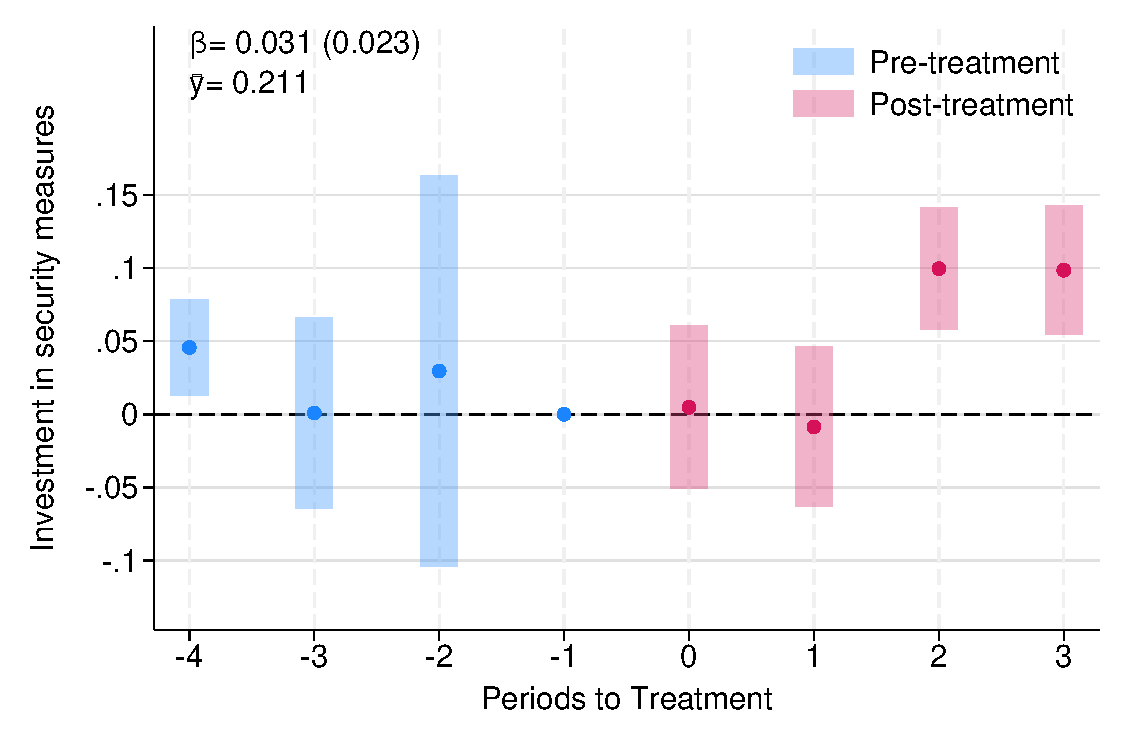
\includegraphics[width=0.98\textwidth]{../manuscript/Graphs/results_spillover_medidas_general_12.pdf}
        \caption{Spillovers on Households adopting security measures}
    \end{subfigure}
    \begin{minipage}{0.95\textwidth}
    \footnotesize
    Notes: This figure presents the geographic spillover effects of \emph{Plan Cuadrante} from early-adopting ENUSC municipalities on their late-adopting ENUSC neighbours, using the ENUSC sample. Panel (a) reports the effect of \emph{Plan Cuadrante} on the probability of household victimization in the last 12-months using the ENUSC survey. Panel (b) reports the effect on crime perception using the ENUSC survey. Panel (c) reports the effect on trust in the police using the ENUSC survey. Panel (d) reports the results on the probability of purchasing private security measures in the last twelve months using the ENUSC survey. The focal treated sample consists of six late-adopting ENUSC municipalities---Molina, Tocopilla, San Carlos, Padre Hurtado, Calera, and Limache---each assigned a spillover-onset date equal to the year its earliest-adopting ENUSC neighbour received \emph{Plan Cuadrante}: Curic\'o (2005) for Molina, Iquique (2005) for Tocopilla, Chill\'an (2007) for San Carlos, Pe\~naflor (2008) for Padre Hurtado, and Quillota (2008) for both Calera and Limache. Estimation is performed using the difference-in-differences estimator for staggered treatment adoption of \citet{Callaway}. The dots represent the estimated dynamic effects and the bars behind them denote 95\% confidence intervals. Standard errors are clustered at the municipality level. The pooled effect  and the mean of the outcome among municipalities with no treated neighbors are reported in each panel.
    \end{minipage}
\end{figure}

